\scanpage{3}

\noindent\begin{minipage}[t]{.34\linewidth}
\(\checkmark\)
\diagram{\begin{tikzcd}[ampersand replacement=\&,column sep=1.5em]
{\unsure{F|\mathbb F}}_0
 \& \mathbb F_1 \arrow[l,shift right=.7ex,"s_1"'] \arrow[l,shift left=.7ex,"t_1"]
 \& \mathbb F_2\mathord{.} \arrow[l,shift right=.7ex,"s_2"'] \arrow[l,shift left=.7ex,"t_2"]
\end{tikzcd}}
\diagram{\begin{tikzcd}[ampersand replacement=\&,column sep=1.5em]
\mathbb F_0 \arrow[r,dash,"\sigma_1", "{\unsure{\cdot|\scriptscriptstyle >}}" description,pos=.97]
 \& f_1 \arrow[r,"\sigma_2"]
 \& F_2
\end{tikzcd}}
\[
\mu^4_1\quad\mu^2_1\quad\mu^2_2
\]
\[
\begin{aligned} &a\\ &\ell\\\ &r\end{aligned}
\]
\end{minipage}\hfill
\begin{minipage}[t]{.64\linewidth}
\figure{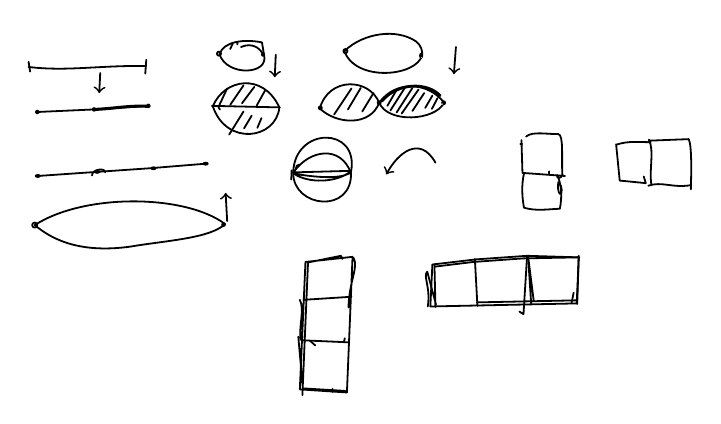
\begin{tikzpicture}[x=.0065cm,y=-.0065cm,line width=.65pt,line cap=round,line join=round]
\draw (723,94)..controls(797,103)and(858,91)..(953,92)
 (723,84)--(726,103) (953,80)--(951,107);
\draw[->] (863,106)--(861,145);
\draw (740,182)--(851,177)--(957,170);
\foreach \x/\y in {740/182,851/177,957/170}{\fill (\x,\y) circle[radius=4.4];}
\draw[line width=1.1pt] (852,177)..controls(895,175)and(917,169)..(958,171);
\draw (1096,69)..controls(1104,44)and(1144,39)..(1179,46)--(1183,70)
 ..controls(1194,110)and(1110,113)..(1096,69);
\draw (1138,55)..controls(1159,46)and(1174,56)..(1181,69);
\draw (1122,48)--(1117,59) (1131,46)--(1131,50);
\draw (1095,68) circle[radius=4];\fill (1181,70) circle[radius=4];
\draw[->] (1206,70)--(1204,114);
\draw (1083,171)..controls(1105,117)and(1181,104)..(1213,173)
 ..controls(1207,235)and(1110,250)..(1083,171);
\draw (1081,170)--(1214,173);
\draw (1111,136)--(1096,168)..controls(1093,172)and(1094,175)..(1097,177) (1143,130)--(1117,168) (1164,133)--(1140,165)
 (1185,140)--(1169,169) (1143,181)--(1115,226) (1159,189)--(1144,214) (1178,194)--(1170,213);
\draw (1340,63)..controls(1379,26)and(1443,19)..(1480,44)
 ..controls(1490,52)and(1493,63)..(1492,71)
 ..controls(1481,113)and(1362,124)..(1340,63);
\draw (1342,63) circle[radius=4];\fill (1490,72) ellipse[x radius=4,y radius=6];\fill[white] (1490.8,75.5) circle[radius=.9];
\draw[->] (1558,55)--(1554,108);
\draw (1292,175)..controls(1310,112)and(1389,116)..(1408,164)
 ..controls(1391,210)and(1325,207)..(1292,175);
\draw (1408,164)..controls(1440,119)and(1504,123)..(1535,164)
 ..controls(1517,199)and(1426,205)..(1408,164);
\draw[line width=1pt] (1413,161)..controls(1445,123)and(1503,124)..(1527,150);
\foreach \x/\y in {1293/174,1408/164}{\fill (\x,\y) circle[radius=4.8];}\fill (1534,164) circle[radius=4.8];\fill[white] (1531.5,166.5) circle[radius=1.2];
\draw (1354,136)--(1320,187) (1372,135)--(1347,177) (1397,145)--(1375,181)
 (1442,139)--(1424,170) (1458,135)--(1430,179) (1473,135)--(1442,183)
 (1485,138)--(1452,185) (1496,145)--(1473,180) (1512,150)--(1498,174) (1522,155)--(1511,176);
\draw (741,307)--(857,299)--(959,292)--(1069,283);
\foreach \x/\y in {741/307,857/299,967/292,1069/283}{\fill (\x,\y) ellipse[x radius=6,y radius=3.8];}
\draw (847,306)..controls(846,294)and(873,290)..(873,300);
\draw (735,403)..controls(833,340)and(1030,343)..(1107,401)
 ..controls(1077,429)and(993,433)..(922,445)
 ..controls(814,460)and(762,425)..(735,403);
\draw (735,403) circle[radius=5];
\fill (1104,402) circle[radius=4.6];
\draw[->] (1111,395)--(1108,340);
\draw (1240,301)..controls(1242,210)and(1370,209)..(1353,299)
 ..controls(1357,382)and(1240,370)..(1240,301);
\draw (1241,299)..controls(1274,254)and(1332,248)..(1352,299)
 (1240,300)--(1352,297) (1242,303)..controls(1271,322)and(1324,320)..(1351,299)
 (1244,303)..controls(1288,310)and(1328,313)..(1350,302);
\draw (1245,294)..controls(1245,289)and(1248,284)..(1251,285)
 (1237,296)..controls(1239,302)and(1235,307)..(1236,314);
\draw[->] (1518,281)..controls(1487,226)and(1444,263)..(1422,304);
\draw (1686,237)--(1688,301)--(1771,307)
 (1695,230)..controls(1707,219)and(1739,226)..(1758,225)
 ..controls(1769,227)and(1764,273)..(1766,305)
 (1740,302)--(1740,298)
 (1691,302)..controls(1686,324)and(1687,348)..(1691,369)
 ..controls(1715,376)and(1736,372)..(1761,371)
 ..controls(1766,347)and(1764,323)..(1756,305);
\draw (1683.8,244.5)--(1687.5,244.5)
 (1756,306)..controls(1753,311)and(1764,313)..(1765,306)
 (1758,319)..controls(1768,328)and(1765,343)..(1761,342)..controls(1757,337)and(1757,328)..(1758,319);
\draw (1871,245)--(1878,316)--(1929,321)--(1925,308)
 (1871,246)..controls(1894,238)and(1917,241)..(1938,241)
 (1935,236)..controls(1946,257)and(1935,296)..(1940,325)
 (1937,238)--(2013,235)..controls(2019,250)and(2018,298)..(2017,333)
 (1934,326)..controls(1961,317)and(1980,331)..(2017,325);
\draw (1264,475)--(1356,465)--(1345,730)--(1253,724)--cycle
 (1260,549)--(1354,543) (1256,628)--(1348,632)
 (1258,735)--(1269,476)--(1333,463)--(1336,469)
 (1358,467)..controls(1368,486)and(1350,509)..(1348,564)
 (1253,549)..controls(1263,567)and(1250,604)..(1255,627)
 (1250,621)--(1259,722)--(1342,727);
\draw (1273,629)--(1283,638) (1339,632)--(1341,624)
 (1317,729)--(1317,723);
\draw (1512,480)--(1597,470)--(1697,463)--(1798,466)--(1794,556)--(1508,562)--cycle
 (1595,469)--(1600,561) (1697,464)--(1690,577)--(1682,572);
\draw (1518,484)--(1592,475)--(1690,468)--(1799,466)
 (1503,562)..controls(1509,524)and(1493,502)..(1502,494)--(1519,558)
 (1518,563)--(1516,480) (1599,554)--(1794,550) (1705,556)--(1699,464)--(1710,551)
 (1784,555)--(1788,535) (1795,557)--(1798,463);
\end{tikzpicture}}
\end{minipage}

% printed form
% Typed address label, running from the bottom toward the top of the sheet.
\noindent\texttt{MR\quad LE PROFESSEUR GROTHENDIECK ALEX.}\\
\texttt{MATHEMATIQUES\unsure{.}\hspace{8em}5}

\[
I_A\,\circ\,\unsure{S|s}\longrightarrow S
\]

\figure{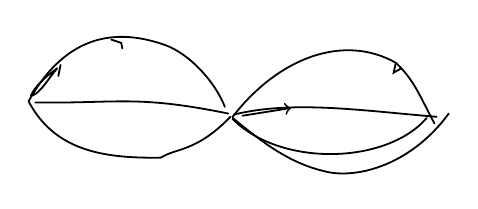
\begin{tikzpicture}[x=.014cm,y=-.014cm,line width=.65pt,line cap=round]
\draw (265,1054)..controls(300,991)and(347,988)..(389,1003)
 ..controls(411,1011)and(434,1036)..(443,1059);
\draw (448,1068)..controls(417,1100)and(399,1096)..(385,1105)
 ..controls(329,1106)and(288,1097)..(265,1054);
\draw (271,1055)..controls(347,1056)and(362,1048)..(446,1065);
\draw (450,1068)..controls(491,1015)and(550,992)..(598,1019)
 ..controls(615,1035)and(620,1050)..(633,1074)
 (646,1065)..controls(610,1114)and(559,1125)..(532,1117)
 ..controls(498,1109)and(471,1086)..(450,1069);
\draw (451,1066)..controls(504,1053)and(564,1062)..(635,1068)
 (450,1070)..controls(494,1114)and(590,1111)..(626,1069);
\draw[->] (459,1067)--(503,1060);
% Small contour returns; their semantic status as arrows is not asserted.
\draw (267,1049)..controls(275,1048)and(283,1033)..(291,1024)
 (291,1024)..controls(280,1032)and(271,1040)..(267,1049)
 (294,1021)--(292,1031)
 (340,998)--(349,1001)--(350,1006)
 (598,1019)--(596,1028)--(603,1024);
\end{tikzpicture}}

\figure{\begin{tikzpicture}[x=.011cm,y=-.011cm,line width=.65pt,line cap=round]
\draw (1326,876)..controls(1346,861)and(1385,870)..(1418,869)--(1439,944)
 (1331,884)--(1345,942)..controls(1348,950)and(1384,947)..(1402,949)--(1398,943)
 (1424,859)--(1515,854)..controls(1535,874)and(1536,912)..(1538,945)
 (1408,956)..controls(1444,943)and(1500,953)..(1542,939)
 (1343,947)..controls(1346,970)and(1348,992)..(1361,1013)
 ..controls(1396,1033)and(1419,1029)..(1445,1016)--(1548,1012)--(1541,944)
 (1435,949)--(1444,1019) (1444,957)--(1445,1011) (1538,998)--(1541,1012);
\fill (1316,870) circle[radius=1.5];\fill (1738,730) circle[radius=1.1];
\draw (1725.7,731)--(1730,731);
\draw (1711,748)--(1725,862) (1716,713)--(1734,775)
 (1709,763)--(1843,753)--(1939,748)--(2043,744)--(2167,739)
 (1725,760)--(1834,762)
 (1838,737)--(1845,770) (1935,735)--(1942,760)
 (2041,735)--(2047,752) (2153,730)--(2153,756) (2163,735)--(2162,746);
\end{tikzpicture}}

\[
\Delta_{n_1}\times\Delta_{n_2}\times
\mathord{-}\,\mathord{-}\,\unsure{<|\times}\,\Delta_{n_n}
\]

\figure{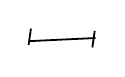
\begin{tikzpicture}[line width=.65pt]
\draw (0,0)--(.85,.04) (0,-.05)--(.03,.16) (.81,-.08)--(.84,.13);
\end{tikzpicture}}

\diagram{\begin{tikzcd}[ampersand replacement=\&,column sep=1.4em,row sep=1em,cells={nodes={inner sep=.4pt}}]
\bullet\arrow[r]\arrow[d,shorten >=3pt] \& {}\arrow[r] \& {}\arrow[r] \& {}\arrow[r] \& \bullet\\
\bullet \& \& \& \&
\end{tikzcd}}

\[
\Delta_{n_1}\times\Delta
\]

\noindent\begin{minipage}{.40\linewidth}
\diagram{\begin{tikzcd}[ampersand replacement=\&,column sep=1.4em,row sep=1.2em,cells={nodes={inner sep=0pt,minimum size=0pt}},
 execute at end picture={\foreach \rowa/\rowb in {1/2,2/3,3/4}{
 \foreach \fracx/\fracy/\low/\high in {.04/.37/.12/.97,.24/.68/.03/.89,.62/.93/.16/.77}{
 \path (\tikzcdmatrixname-\rowb-1.center)--(\tikzcdmatrixname-\rowb-2.center) coordinate[pos=\fracx] (hatchlo);
 \path (\tikzcdmatrixname-\rowa-1.center)--(\tikzcdmatrixname-\rowa-2.center) coordinate[pos=\fracy] (hatchhi);
 \path (hatchlo)--(hatchhi) coordinate[pos=\low] (inklo) coordinate[pos=\high] (inkhi);
 \draw[line width=.33pt] (inklo)--(inkhi);}}}]
{}\arrow[r]\arrow[d,dash] \& {}\arrow[r]\arrow[d,dash] \& {}\arrow[r]\arrow[d,dash] \& {}\arrow[r]\arrow[d,dash] \& {}\arrow[d,dash]\\
{}\arrow[r]\arrow[d,dash] \& {}\arrow[r]\arrow[d,dash] \& {}\arrow[r]\arrow[d,dash] \& {}\arrow[r]\arrow[d,dash] \& {}\arrow[d,dash]\\
{}\arrow[r]\arrow[d,dash] \& {}\arrow[r]\arrow[d,dash] \& {}\arrow[r]\arrow[d,dash] \& {}\arrow[r,shorten <=2pt,shorten >=2pt]\arrow[d,dash] \& {}\arrow[d,dash]\\
{}\arrow[r] \& {}\arrow[r] \& {}\arrow[r] \& {}\arrow[r,shorten <=2pt,shorten >=2pt] \& {}
\arrow[from=1-1,to=2-2,draw=none,"\Downarrow" description]
\arrow[from=1-2,to=2-3,draw=none,"\Downarrow" description]
\arrow[from=1-3,to=2-4,draw=none,"\Downarrow" description]
\arrow[from=1-4,to=2-5,draw=none,"\Downarrow" description]
\arrow[from=2-1,to=3-2,draw=none,"\Downarrow" description]
\arrow[from=2-2,to=3-3,draw=none,"\Downarrow" description]
% The middle-row third cell has two heavy descending strokes, no secure head.
\arrow[from=2-3,to=3-4,draw=none,"{\vcenter{\hbox{\begin{tikzpicture}[x=.55em,y=.55em,line width=.65pt]\draw (0,1.1)--(0,0) (.23,1.1)--(.23,0);\end{tikzpicture}}}}" description]
\arrow[from=2-4,to=3-5,draw=none,"\Downarrow" description]
\arrow[from=3-1,to=4-2,draw=none,"\Downarrow" description]
\arrow[from=3-2,to=4-3,draw=none,"\Downarrow" description]
\arrow[from=3-3,to=4-4,draw=none,"\Downarrow" description]
\arrow[from=3-4,to=4-5,draw=none,"\Downarrow" description]
\arrow[from=1-1,to=4-1,shift left=.22ex,shorten >=4pt]
\arrow[from=1-2,to=4-2,dash,shift right=.3ex]
\arrow[from=1-3,to=4-3,dash,shift right=.3ex]
\arrow[from=1-4,to=4-4,dash,shift right=.3ex]

\end{tikzcd}}
\end{minipage}\hfill
\begin{minipage}{.58\linewidth}
\figure{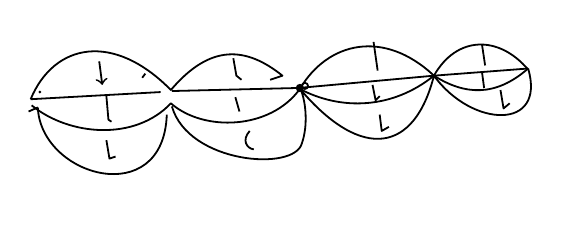
\begin{tikzpicture}[x=.013cm,y=-.013cm,line width=.65pt,line join=round]
\draw (1010,1405)..controls(1033,1350)and(1091,1339)..(1147,1396)
 ..controls(1186,1350)and(1221,1354)..(1256,1382)--(1244,1386)
 (1273,1395)..controls(1300,1349)and(1355,1336)..(1404,1382)
 ..controls(1426,1343)and(1467,1342)..(1496,1376);
\draw (1010,1405)--(1137,1398)
 (1148,1397)--(1272,1394)--(1404,1382)--(1496,1375);
\fill (1019,1398) circle[radius=1.5];
\draw (1122,1380)--(1119,1384)
 (1008,1417)--(1017,1413);
\draw (1278,1392) circle[radius=3];
\draw (1011,1411)..controls(1048,1441)and(1112,1446)..(1147,1409)
 ..controls(1179,1437)and(1244,1435)..(1273,1395)
 ..controls(1313,1416)and(1363,1415)..(1404,1382)
 ..controls(1434,1401)and(1464,1403)..(1496,1375);
\draw (1017,1413)..controls(1020,1481)and(1140,1514)..(1143,1420)
 (1148,1412)..controls(1164,1468)and(1268,1476)..(1275,1448)
 ..controls(1281,1431)and(1279,1408)..(1274,1396)
 ..controls(1334,1466)and(1385,1457)..(1404,1382)
 ..controls(1441,1433)and(1514,1436)..(1496,1375);
\fill (1273,1394) circle[radius=4];
\draw[->] (1077,1368)--(1080,1391);
\draw (1084,1402)--(1086,1425)--(1089,1427) (1084,1445)--(1087,1463)--(1093,1461)
 (1208,1365)--(1211,1382)--(1216,1386) (1210,1403)--(1214,1417)
 (1224,1436)..controls(1216,1445)and(1221,1453)..(1228,1454)
 (1345,1349)--(1349,1377) (1344,1391)--(1347,1406)--(1351,1402)
 (1351,1420)--(1353,1436)--(1360,1432)
 (1451,1352)--(1454,1372) (1451,1379)--(1453,1394)
 (1469,1396)--(1472,1414)--(1478,1409);
\end{tikzpicture}}
\end{minipage}

\[
\vcenter{\hbox{
\begin{tikzpicture}[x=.85em,y=.85em,line width=.38pt,baseline]\draw (0,0)--(.59,.92)--(.82,0)--cycle;\draw (.09,.03)--(.69,.96);\end{tikzpicture}}}_n\times\vcenter{\hbox{
\begin{tikzpicture}[x=.85em,y=.85em,line width=.38pt,baseline]\draw (0,0)--(.59,.92)--(.82,0)--cycle;\draw (.09,.03)--(.69,.96);\end{tikzpicture}}}_{n'}
\]
\[
\begin{aligned}
\mathbb F_0 &= \mathrm{Ob}\,\Delta_{\unsure{kn'|n\,n'|n'}}\\
F_1 &= \deleted{\unsure{\mathrm{Ob}\,\Delta_n|\mathrm{O}\Delta_n}}\deleted{\unsure{\mathrm{Ob}}}{\unsure{\mathbb F|F}}\mathrm{l}^{\unsure{\prime}}(\Delta_n)\times\mathrm{Ob}\,\Delta_{n'}\\
F &\mathrel{\unsure{-|=}} \mathbb F\mathrm{l}\,(\Delta_n)\times\mathbb F\mathrm{l}\,\Delta_{n''})
\end{aligned}
\]
% The detached stroke after live l is prime-like; an isolated pen mark remains possible.
% The lower line has no visible subscript after the initial F and only one visible relation bar.
% The second closing parenthesis has no visible matching opening parenthesis.
% A separate long ink stroke runs toward the right edge beneath the end of this line.
\figure{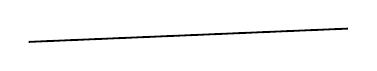
\begin{tikzpicture}[x=.013cm,y=-.013cm,line width=.65pt]
\draw (2040,1652)--(2352,1639);
\end{tikzpicture}}
% archive sheet number: 2
